\section{stabilizer.h File Reference}
\label{stabilizer_8h}\index{stabilizer.h@{stabilizer.h}}


This graph shows which files directly or indirectly include this file:\begin{figure}[H]
\begin{center}
\leavevmode
\includegraphics[width=111pt]{stabilizer_8h__dep__incl}
\end{center}
\end{figure}
\subsection*{Defines}
\begin{CompactItemize}
\item 
\#define {\bf PI}~3.14
\item 
\#define {\bf GYRO1\_\-ZERO\_\-VALUE}~-65.0
\item 
\#define {\bf GYRO\_\-TO\_\-OMEGA\_\-FACTOR}~0.002556634
\item 
\#define {\bf ACCL\_\-TO\_\-DEGREE\_\-FACTOR}~25.0
\item 
\#define {\bf STEERING\_\-ZERO\_\-POINT}~512
\item 
\#define {\bf STEERING\_\-RESPONSIVENESS}~0.001
\item 
\#define {\bf K\_\-ANGLE}~5.0
\item 
\#define {\bf K\_\-OMEGA}~0.16666
\item 
\#define {\bf K\_\-CORR\_\-FACTOR}~1.0
\item 
\#define {\bf SET\_\-POINT}~0.0
\item 
\#define {\bf CUR\_\-SPEED\_\-FACTOR}~4.0
\end{CompactItemize}
\subsection*{Functions}
\begin{CompactItemize}
\item 
void {\bf stabilizer\_\-loop} (void)
\end{CompactItemize}


\subsection{Define Documentation}
\index{stabilizer.h@{stabilizer.h}!ACCL_TO_DEGREE_FACTOR@{ACCL\_\-TO\_\-DEGREE\_\-FACTOR}}
\index{ACCL_TO_DEGREE_FACTOR@{ACCL\_\-TO\_\-DEGREE\_\-FACTOR}!stabilizer.h@{stabilizer.h}}
\subsubsection{\setlength{\rightskip}{0pt plus 5cm}\#define ACCL\_\-TO\_\-DEGREE\_\-FACTOR~25.0}\label{stabilizer_8h_64d51047e317d0d7da457f60bcd47028}


correction factor for scaling the acclerometer value to degrees 

Definition at line 72 of file stabilizer.h.

Referenced by stabilizer\_\-loop().\index{stabilizer.h@{stabilizer.h}!CUR_SPEED_FACTOR@{CUR\_\-SPEED\_\-FACTOR}}
\index{CUR_SPEED_FACTOR@{CUR\_\-SPEED\_\-FACTOR}!stabilizer.h@{stabilizer.h}}
\subsubsection{\setlength{\rightskip}{0pt plus 5cm}\#define CUR\_\-SPEED\_\-FACTOR~4.0}\label{stabilizer_8h_a4a6a13b91688973362edab491ec5801}


factor to scale the set value with for current speed TODO: Check comment! Add detailed desciption 

Definition at line 104 of file stabilizer.h.

Referenced by stabilizer\_\-loop().\index{stabilizer.h@{stabilizer.h}!GYRO1_ZERO_VALUE@{GYRO1\_\-ZERO\_\-VALUE}}
\index{GYRO1_ZERO_VALUE@{GYRO1\_\-ZERO\_\-VALUE}!stabilizer.h@{stabilizer.h}}
\subsubsection{\setlength{\rightskip}{0pt plus 5cm}\#define GYRO1\_\-ZERO\_\-VALUE~-65.0}\label{stabilizer_8h_23edd713eb04c1f7b66eec97a198adb0}


the initial value, the gyroscope 1 measures, when not beeing moved 

Definition at line 55 of file stabilizer.h.

Referenced by stabilizer\_\-loop().\index{stabilizer.h@{stabilizer.h}!GYRO_TO_OMEGA_FACTOR@{GYRO\_\-TO\_\-OMEGA\_\-FACTOR}}
\index{GYRO_TO_OMEGA_FACTOR@{GYRO\_\-TO\_\-OMEGA\_\-FACTOR}!stabilizer.h@{stabilizer.h}}
\subsubsection{\setlength{\rightskip}{0pt plus 5cm}\#define GYRO\_\-TO\_\-OMEGA\_\-FACTOR~0.002556634}\label{stabilizer_8h_2963d2e1ade8f16b08002541372d0ed2}


scaling factor to calculate the angular speed (omega) from the Gyroscope1 value

from orignal code : OMEGA = ( ( (GYRO-GYRO\_\-zero) / 2048) $\ast$ 2 $\ast$ PI $\ast$ 300) / 360; $<$=$>$ OMEGA = ( (GYRO-GYRO\_\-zero) $\ast$ 0.920388) / 360 $<$=$>$ OMEGA = ( (GYRO-GYRO\_\-zero) $\ast$ 2.556634E-3

TODO: Needs to be adapted to sensor 

Definition at line 67 of file stabilizer.h.

Referenced by stabilizer\_\-loop().\index{stabilizer.h@{stabilizer.h}!K_ANGLE@{K\_\-ANGLE}}
\index{K_ANGLE@{K\_\-ANGLE}!stabilizer.h@{stabilizer.h}}
\subsubsection{\setlength{\rightskip}{0pt plus 5cm}\#define K\_\-ANGLE~5.0}\label{stabilizer_8h_aeb0d289a6c0bcd92cf00d9ba462d816}


tilt angle factor for kalman algorithm TODO: add detailed description here! This is not documented in original code 

Definition at line 86 of file stabilizer.h.

Referenced by stabilizer\_\-loop().\index{stabilizer.h@{stabilizer.h}!K_CORR_FACTOR@{K\_\-CORR\_\-FACTOR}}
\index{K_CORR_FACTOR@{K\_\-CORR\_\-FACTOR}!stabilizer.h@{stabilizer.h}}
\subsubsection{\setlength{\rightskip}{0pt plus 5cm}\#define K\_\-CORR\_\-FACTOR~1.0}\label{stabilizer_8h_a00a85617f61edf3a55ce70ca5261da0}


correction factor for kalman algorithm TODO: add detailed description here! This is not documented in original code 

Definition at line 96 of file stabilizer.h.\index{stabilizer.h@{stabilizer.h}!K_OMEGA@{K\_\-OMEGA}}
\index{K_OMEGA@{K\_\-OMEGA}!stabilizer.h@{stabilizer.h}}
\subsubsection{\setlength{\rightskip}{0pt plus 5cm}\#define K\_\-OMEGA~0.16666}\label{stabilizer_8h_df0bd5f884ff5fc0e120a13d9de4afac}


angular speed (omega) factor for kalman algorithm TODO: add detailed description here! This is not documented in original code 

Definition at line 91 of file stabilizer.h.

Referenced by stabilizer\_\-loop().\index{stabilizer.h@{stabilizer.h}!PI@{PI}}
\index{PI@{PI}!stabilizer.h@{stabilizer.h}}
\subsubsection{\setlength{\rightskip}{0pt plus 5cm}\#define PI~3.14}\label{stabilizer_8h_598a3330b3c21701223ee0ca14316eca}


PI ... 

Definition at line 52 of file stabilizer.h.

Referenced by stabilizer\_\-loop().\index{stabilizer.h@{stabilizer.h}!SET_POINT@{SET\_\-POINT}}
\index{SET_POINT@{SET\_\-POINT}!stabilizer.h@{stabilizer.h}}
\subsubsection{\setlength{\rightskip}{0pt plus 5cm}\#define SET\_\-POINT~0.0}\label{stabilizer_8h_513c42d8dbcacf9f9f7dde6914a496f5}


setpoint (sollwert) of the controlling algorithm TODO: Check comment! Add detailed desciption 

Definition at line 100 of file stabilizer.h.

Referenced by stabilizer\_\-loop().\index{stabilizer.h@{stabilizer.h}!STEERING_RESPONSIVENESS@{STEERING\_\-RESPONSIVENESS}}
\index{STEERING_RESPONSIVENESS@{STEERING\_\-RESPONSIVENESS}!stabilizer.h@{stabilizer.h}}
\subsubsection{\setlength{\rightskip}{0pt plus 5cm}\#define STEERING\_\-RESPONSIVENESS~0.001}\label{stabilizer_8h_8366037faafd04166b46051a38ad1586}




Definition at line 81 of file stabilizer.h.

Referenced by stabilizer\_\-loop().\index{stabilizer.h@{stabilizer.h}!STEERING_ZERO_POINT@{STEERING\_\-ZERO\_\-POINT}}
\index{STEERING_ZERO_POINT@{STEERING\_\-ZERO\_\-POINT}!stabilizer.h@{stabilizer.h}}
\subsubsection{\setlength{\rightskip}{0pt plus 5cm}\#define STEERING\_\-ZERO\_\-POINT~512}\label{stabilizer_8h_a49e35e5eba9ca864421e9019238d346}


zero point of the steering potentiometer. (10Bit resolution -$>$ 1024 max, so 1024/2) 

Definition at line 78 of file stabilizer.h.

Referenced by stabilizer\_\-loop().

\subsection{Function Documentation}
\index{stabilizer.h@{stabilizer.h}!stabilizer_loop@{stabilizer\_\-loop}}
\index{stabilizer_loop@{stabilizer\_\-loop}!stabilizer.h@{stabilizer.h}}
\subsubsection{\setlength{\rightskip}{0pt plus 5cm}void stabilizer\_\-loop (void)}\label{stabilizer_8h_cc3a7bb7e4532b65fe366e14f3778f86}




Definition at line 45 of file stabilizer.c.

References accl\_\-high\_\-samples, accl\_\-low\_\-samples, ACCL\_\-SAMPLES\_\-BUFSIZE, ACCL\_\-TO\_\-DEGREE\_\-FACTOR, adc\_\-sel\_\-channel(), ADC\_\-STEERING\_\-1, CUR\_\-SPEED\_\-FACTOR, gyro1\_\-samples, GYRO1\_\-SAMPLES\_\-BUFSIZE, GYRO1\_\-ZERO\_\-VALUE, GYRO\_\-TO\_\-OMEGA\_\-FACTOR, K\_\-ANGLE, K\_\-OMEGA, PI, PWM\_\-RESOLUTION, read\_\-adc(), set\_\-motor1(), set\_\-motor2(), SET\_\-POINT, STEERING\_\-RESPONSIVENESS, STEERING\_\-ZERO\_\-POINT, and uart\_\-puts().

Here is the call graph for this function:\begin{figure}[H]
\begin{center}
\leavevmode
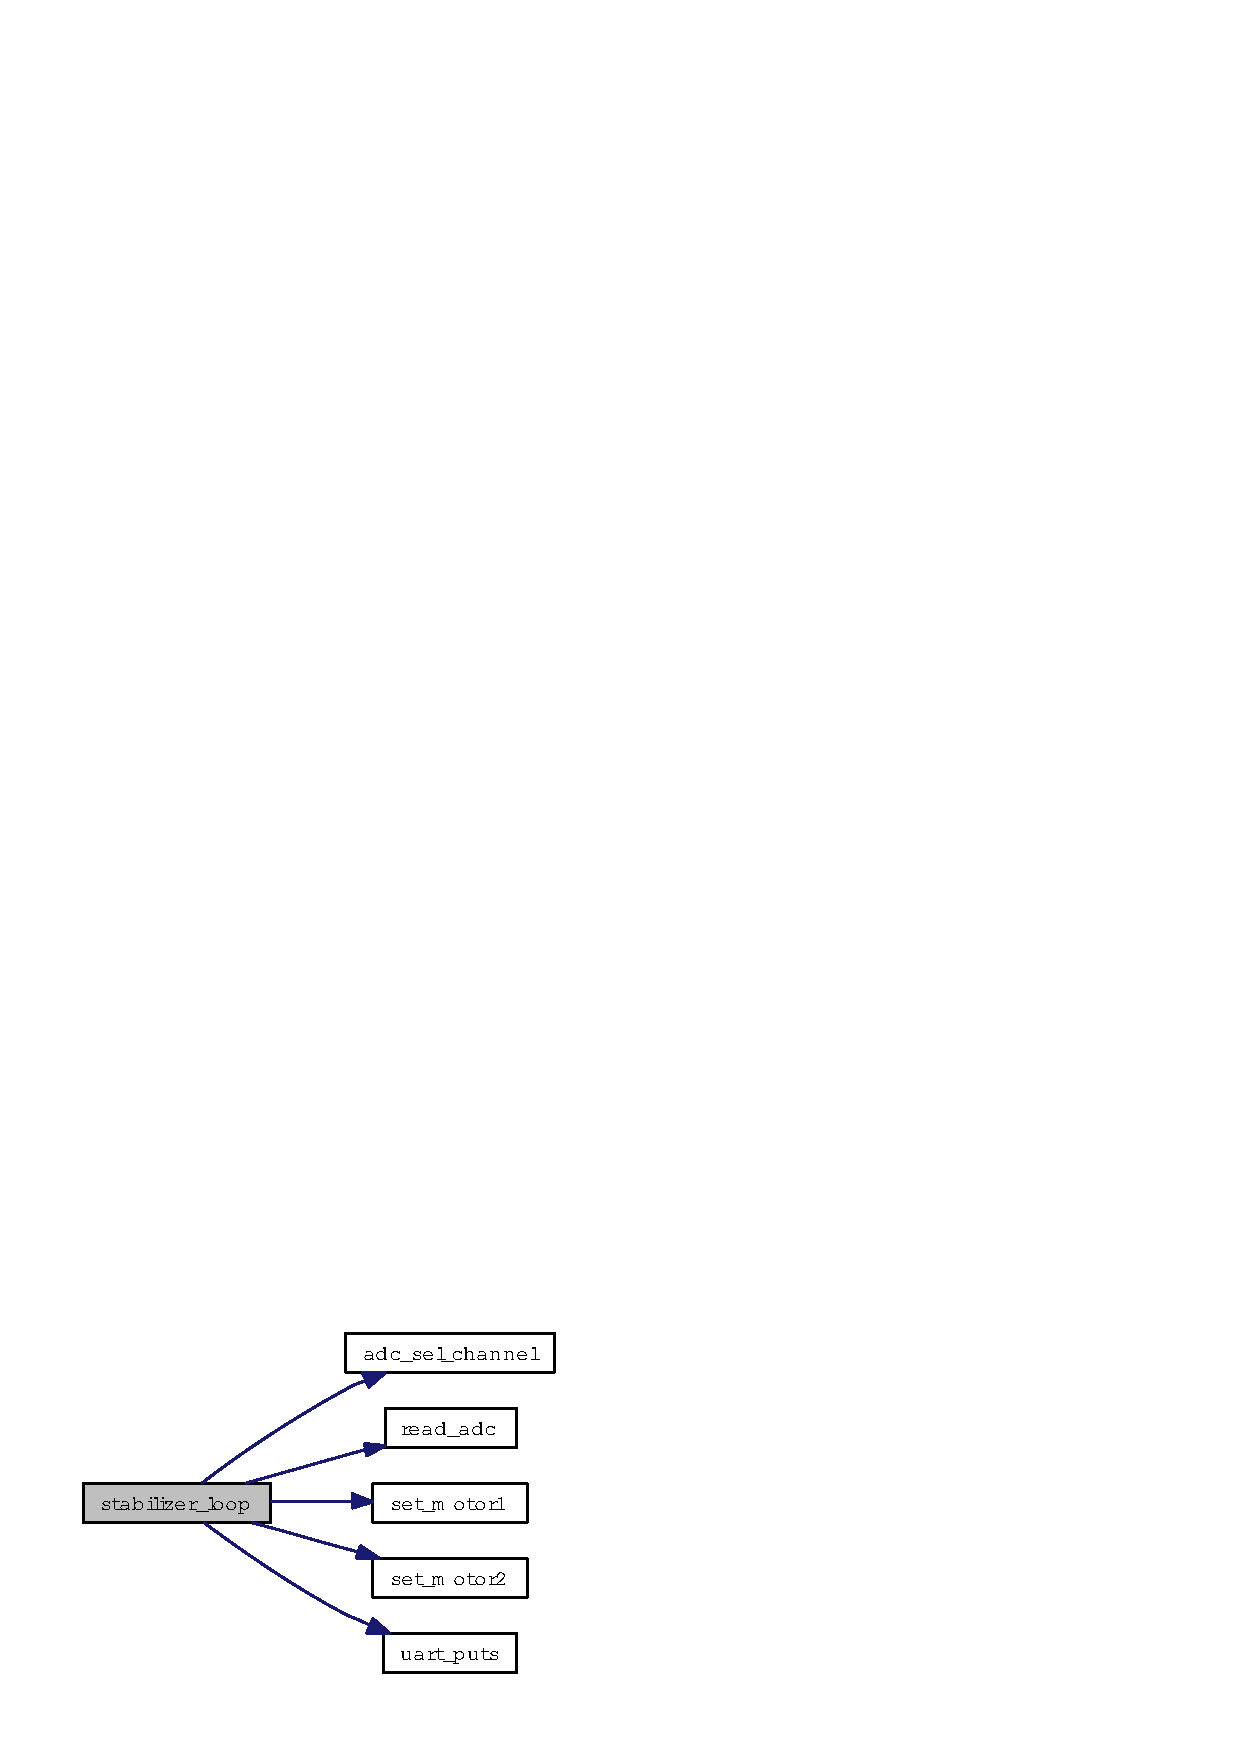
\includegraphics[width=135pt]{stabilizer_8h_cc3a7bb7e4532b65fe366e14f3778f86_cgraph}
\end{center}
\end{figure}
